\documentclass[12pt,oneside,slovak,a4paper]{article}
\usepackage[slovak]{babel}
\usepackage[utf8]{inputenc}
\usepackage[T1]{fontenc}
\usepackage{graphicx}
\usepackage{listings}
\usepackage{url} % príkaz \url na formátovanie URL
\usepackage{hyperref} % odkazy v texte budú aktívne (pri niektorých triedach dokumentov spôsobuje posun textu)
\usepackage{longtable} 
\usepackage{cite}
\usepackage{times}
\usepackage{listings} % umožňuje paste kódu \lstset{language=Java} \begin{lstlisting}[frame=single]
\usepackage[dvips,dvipdfm,a4paper,centering,textwidth=14cm,top=4.6cm,headsep=.6cm,footnotesep=1cm,footskip=0.6cm,bottom=3.8cm]{geometry}
%opening
\pagestyle{headings}
\title{Objektovo orientované programovanie\linebreak Správa o realizácií projektu}

\author{Michal Kováčik\\[2pt]
	{\small Slovenská technická univerzita v Bratislave}\\
	{\small Fakulta informatiky a informačných technológií}\\
	{\small \texttt{xkovacikm2@gmail.com}}
	}

\date{\small 5. máj 2015}

\begin{document}

\maketitle

\pagebreak
\section{Spresnenie rámcového zadania}
\subsection{Popis tried a ich interakcia}
Vo svojom projekte na Objektovo Orientované Programovanie chcem vytvoriť simuláciu bitky 2 tankových plukov v generovanej mape.
Každý pluk má svojho vrchného veliteľa, ktorý posiela správu veliteľom jednotlivých tankov, kam v mape je potrebné sa dostať, aby sa bitka vyhrala (cieľom môže byť dostať sa na určité miesto na mape, ako zjednodušený capture the flag, alebo zničiť všetky nepriateľské tanky).
Každý tank má posádku 3 ľudí v zložení veliteľ tanku, vodič tanku a strelec a samotný tank sa skladá z tela tanku a zo streleckej veže. Ďalej by som popísal úlohy jednotlivých členov posádky a častí tanku.

\paragraph{Veliteľ tanku} je hlavným medzičlánkom medzi veliteľom pluku a ostatnými členmi posádky. Príjma rozkazy od veliteľa pluku, o súradniciach cieľa, kam je potrebné sa dostať, zistí ako sa tam dostať a krok po kroku naviguje vodiča kadiaľ treba ísť. Zároveň kontroluje, či sa na obzore tanku nenachádza nepriateľský tank, a v prípade, že sa nachádza, dáva strelcovi pokyn strieľať na súradnice nepriateľského tanku.

\paragraph{Vodič} sa stará smerovanie pohybu tanku na súradnice políčka zadaného veliteľom tanku, tzn. zistí, či je potrebné ísť nahor, nadol, vpravo, alebo vľavo aby sa na dané súradnice dostal. Takisto veliteľa informuje o úspechu/neúspechu presunu (v ceste sa môže ocitnúť prekážka, napr. iný tank). V prípade neúspechu veliteľ prepočíta trasu.

\paragraph{Strelec} sa stará o smerovanie streleckej veže tanku. Keď veliteľ tanku dá pokyn strieľať na súradnice výskytu nepriateľa, tak strelec zistí do ktorého smeru je potrebné natočiť vežu (nezávisle od pohybu tanku) a tým smerom vystrelí.

\paragraph{Telo tanku} je ''hmotný'' objekt, to znamená, že nie je schopný prechádzať cez steny mapy a takisto po zásahu strelou by sa mal oslabiť/zničiť spolu s celou posádkou. Je schopný pohybovať sa smerom, ktorý mu určí vodič tanku.

\paragraph{Veža tanku} je súčasťou tanku. Jej úlohou je vystreľovať projektily smerom, ktorý jej určí strelec. Pohybuje sa zároveň s tankom, ale smerovať projektily môže nezávisle od smerovania tanku

\paragraph{Projektil} je vytváraný vežou tanku. Po výstrele je to samostatný objekt, ktorý ďalej už nemá nič spoločné s tankom, ktorý ju vystrelil. Má smer a rýchlosť, ktoré mu boli udelené vežou tanku pri výstrele. Má určitý dolet, ktorý keď prekročí, alebo keď narazí do iného ''hmotného'' objektu (stena/tank/iný projektil) tak sa zničí.

\paragraph{Observer} sa stará o sledovanie kolízií pohybujúcich sa objektov po mape.

\subsection{Stanovenie cieľov}
Po dokončení by mal program byť schopný vykreslovať simuláciu v jednoduchom 2D grafickom prostredí. Uživateľ by mal byť schopný označiť si ľubovoľný tank a prebrať úlohu ľubovoľného člena posádky, tzn. napríklad ako vodič bude schopný ovládať pohyb tanku, ako veliteľ môže strelcovi zadávať ciele na strelbu a vodičovi zadávať súradnice pohybu, a ako strelec môže ľubovoľne strieľať ľubovoľným smerom projektily.

\section{Štruktúra systému}
\subsection{Diagram}
Diagram v SVG formáte nájdete v zložke s odovzdanými súbormi.
\begin{center}
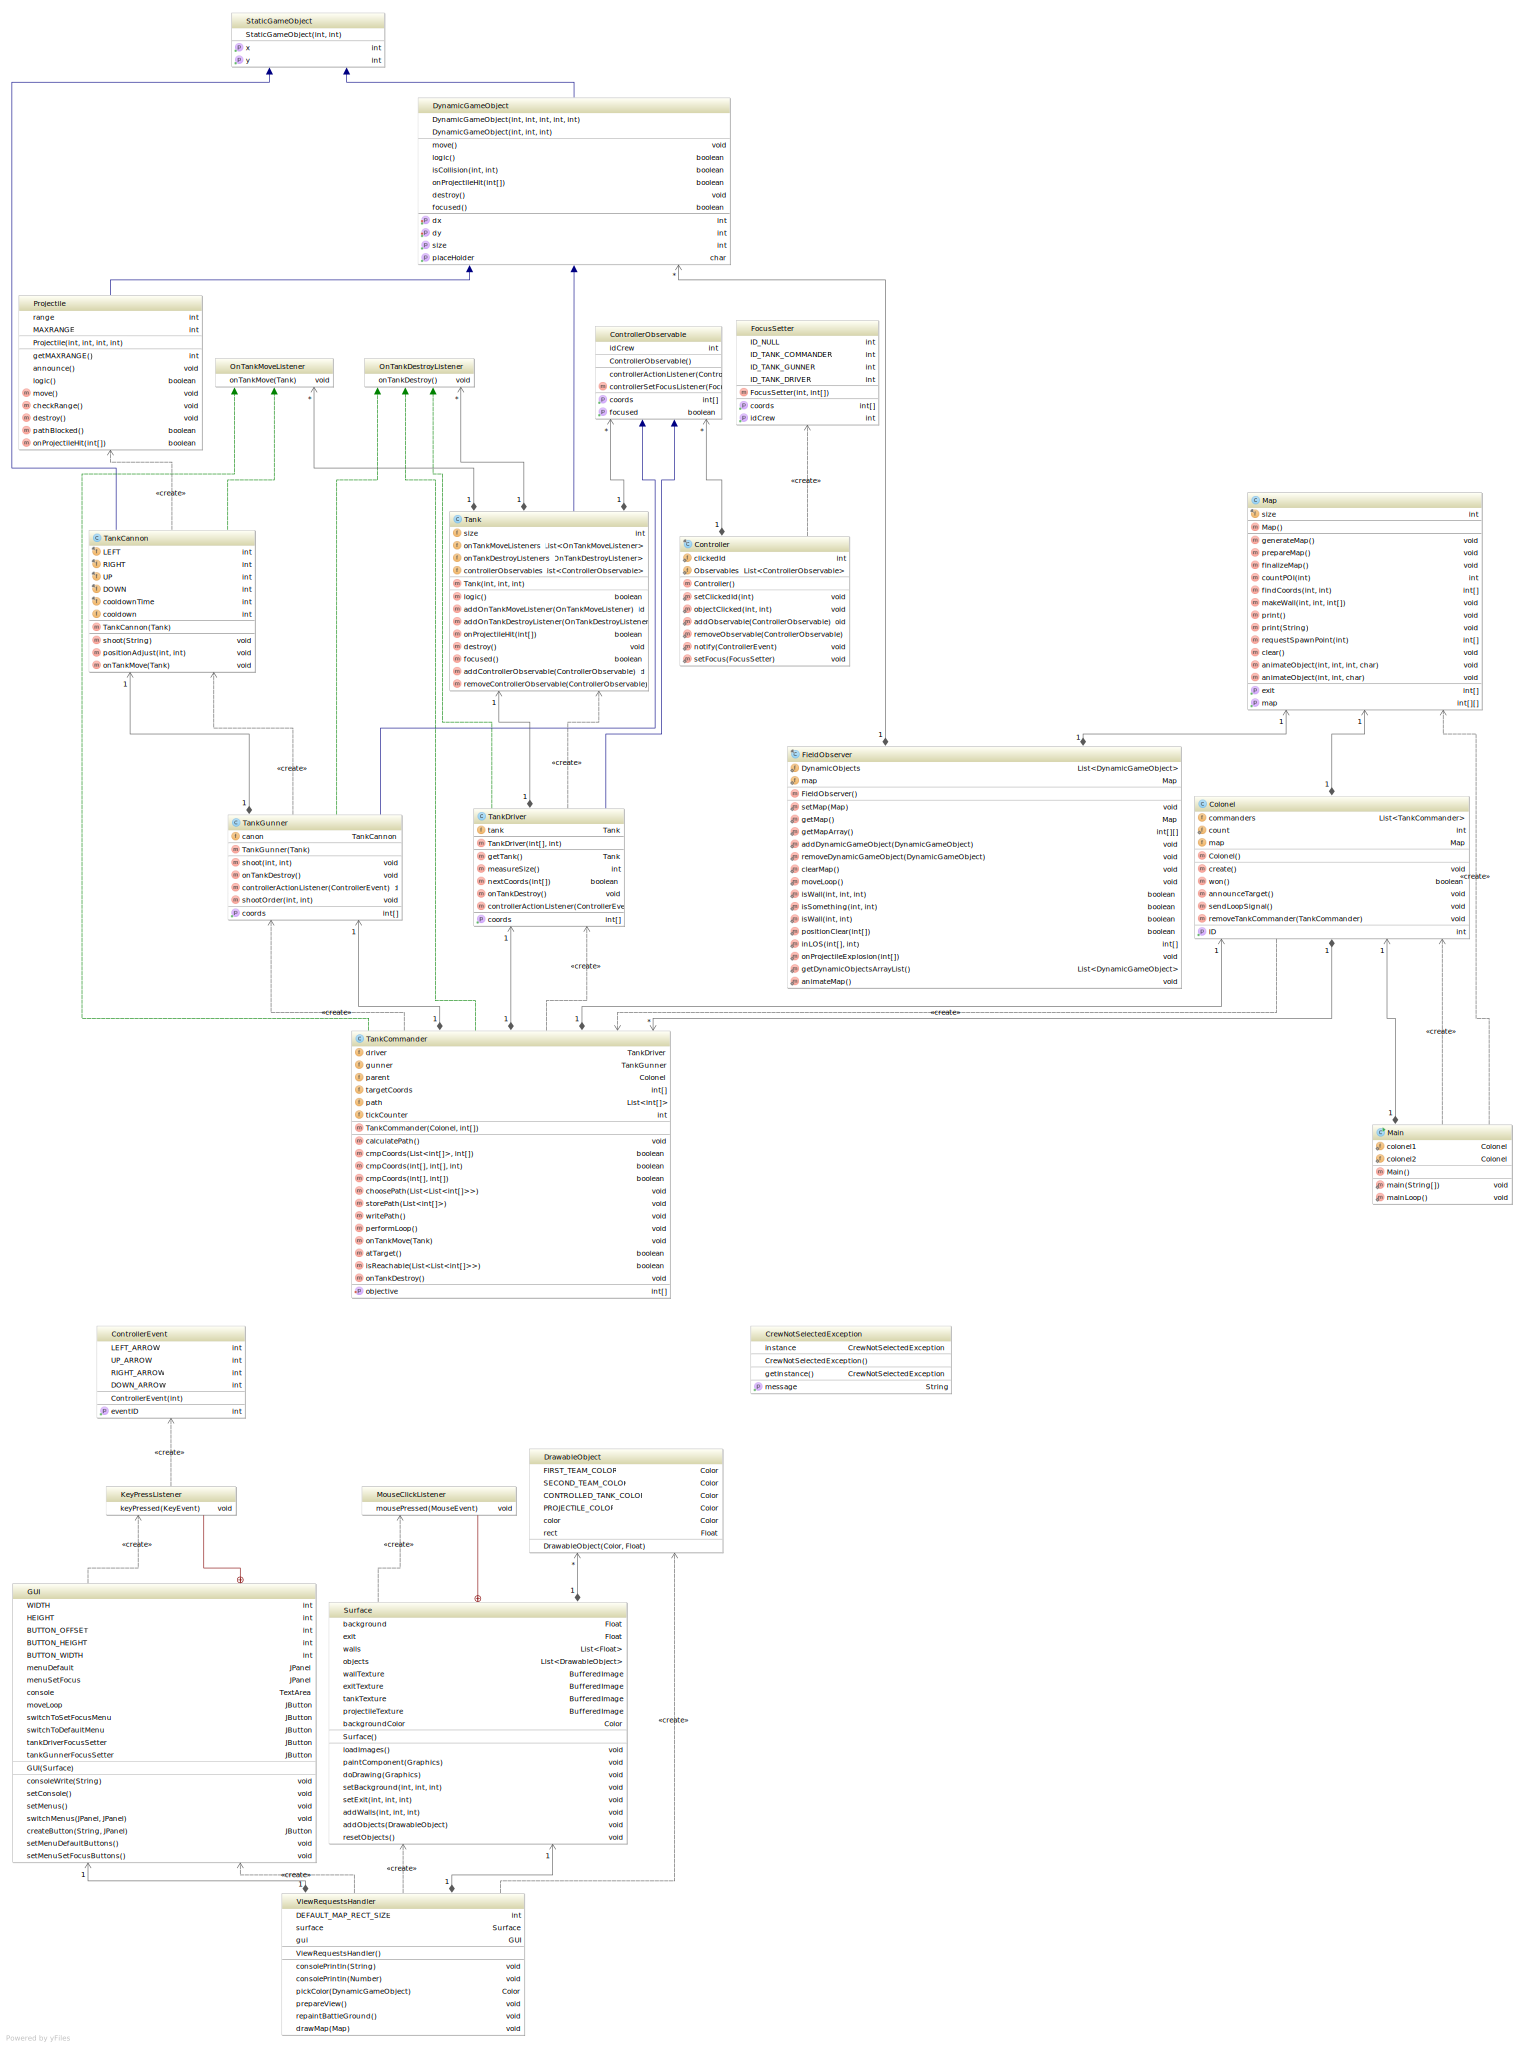
\includegraphics[scale=0.19]{diagram.png}
\end{center}
\subsection{Popis hlavných tried a ich vzťahy}
\subsubsection{Balík model}
Pôjdem v abecednom poradí cez podbalíky a v abecednom poradí popíšem všetky triedy z podbalíka, tak ako sú v zložke src
\paragraph{Trieda DynamiGameObject} je abstraktná trieda, ktorá tvorí abstrakciu pre každý pohybujúci sa objekt na mape. Obsahuje metódy pre pohyb, atribúty ako rýchlosť v danom smere a znak, ktorým je reprezentovaný v 2D mape. Priamo v konštruktore sa prihlasuje do observera na pozorovanie.
\paragraph{Trieda StaticGameObject} je abstraktná trieda, ktorá tvorí abstrakciu pre každý objekt, ktorý potrebuje jestvovať v mape na svojich súradniciach. Obsahuje settery na súradnice, a atribúty pre reprezentáciu polohy v priestore
\paragraph{Trieda Main} je hlavnou triedou programu. Vytvára inštanciu mapy, vytvára dvoch plukovníkov a obsahuje metódu moveLoop, ktorá je srdcom programu.
\paragraph{Trieda Colonel} je vrchný veliteľ tankového pluku. Po svojom vytvorení si vytvorí armádu 5 veliteľov tanku. Následne veliteľom pošle informáciu o tom, kde sa nachádza cieľ, ktorý je pre výhru nutné dosiahnuť. Takisto všetkých veliteľov tankov na vlastnom threade informuje o tom, že je nutné vykonať ťah.
\paragraph{Trieda FieldObserver} je observerom modelu. Je to statická trieda, ktorá pri pokuse vytvoriť inštanciu vyhodí výnimku. Obsahuje arraylist všetkých dynamických objektov, takisto obsahuje referenciu na singleton mapy. Každému dynamickému objektu posiela informáciu o nutnosti vykonať pohyb, takisto spracúva otázky dynamických objektov o vzájomných kolíziách.
\paragraph{Trieda TankCommander} je veliteľom tanku. Je spawnovaný Colonelom a vytvára svojich podriadených TankDrivera a TankGunnera. Na základe príkazu od Colonela nastavuje svoj cieľ, kde je nutné sa dostať v mape, aby sa vyhrala bitka. Je zodpovedný za výpočet trasy, keďže ako jediný vlastní referenciu na singleton mapy. Takisto implementuje onTankMoveListener, kde pri volaní metódy toho funkčného interfacu zistí, či sa v okolí nenachádza nepriateľ na ktorého nutné strieľať. Ak ho zbadá, dáva pokyn strelcovi, že na daných súradniciach sa nachádza nepriateľ a je nutné strieľať (viz. výpisy v konzole pri spustení). Ďalej implementuje onTankDestroyListener, ho po zavolaní zabije, rozumej, odhlási všetky jeho referencie v programe a nechá sa zobrať garbage collectorom.
\paragraph{Trieda TankDriver} je vodičom tanku. V každom ťahu spracúva pokyn od veliteľa, na ktoré súradnice sa treba posunúť a on základe terajších a cieľových súradníc nastaví tanku vektory pohybu. V konštruktore vytvára tank, ktorý potom ovláda - je jeho atribútom. Trieda extenduje ControllerObservable, ktorá mu umožňuje spracúvať eventy od Controllera a teda je možné, aby uživateľ prevzal na seba jeho úlohy. Ďalej implementuje onTankDestroyListener, ho po zavolaní zabije, rozumej, odhlási všetky jeho referencie v programe a nechá sa zobrať garbage collectorom.
\paragraph{Trieda TankGunner} je strelcom z veže tanku. Keď dostane od veliteľa pokyn, nastaví vektory aké sa majú vystrelenej strele priradiť (alegóriou by mohlo byť natočenie kanóna do správneho smeru), a zavolá metódu kanónu, ktorá na základe strelcom zadaných parametrov vytvorí objekt projektil. Trieda extenduje ControllerObservable, ktorá mu umožňuje spracúvať eventy od Controllera a teda je možné, aby uživateľ prevzal na seba jeho úlohy. Ďalej implementuje onTankDestroyListener, ho po zavolaní zabije, rozumej, odhlási všetky jeho referencie v programe a nechá sa zobrať garbage collectorom.
\paragraph{Trieda Projectile} je projektil, ktorý spawnuje veža tanku spôsobom, aký jej určite TankGunner. Extenduje DynamicGameObject. Pri kolízií s hocijakým objektom nachádzajúcim sa na mape exploduje a oznámi observeru súradnice miesta svojej explózie. Observer následne oznámi všetkým dynamickým objektom, že nastal na danom mieste výbuch. Má rozmer 1 a rýchlosť pohybu 4 za 1 ťah. Na surface je vykreslovaný ako fialová gulička. 
\paragraph{Trieda Tank} extenduje dynamický objekt. Na surface je vykreslovaný obrázkom tanku a je podfarbený farbou svojho tímu. Pri každom pohybe si tank skúša, či by náhodou nenarazil do steny, v takom prípade odmietne pohyb vykonať. Tank obsahuje zoznam onTankDestroyListenerov, ktorým, pri svojom zničení volá metódu onTankDestroy. Ďalej obsahuje zoznam onTankMoveListenerov, ktorým po každom svojom pohybe volá metódu onTankMove. Ďalej obsahuje list ControllerObservables, kde v každom ťahu kontroluje focus členov posádky, aby ho bolo možné na Surfaci farebne odlíšiť od ostatných, nefocusovaných. V prípade, že sa tank nachádza v blízkosti explózie, tak sa zničí.
\paragraph{TankCanon} extenduje statický objekt. Je schopný spawnovať projektily v smere, ktorý mu určí TankGunner. Implementuje onTankMoveListener, ktorý po každom pohybe tanku upraví jeho pozíciu, aby sa pohyboval spoločne s tankom.
\paragraph{Map} je singleton, teda existuje jej práve jedna inštancia. Je schopná procedurálne vygenerovať terén tak, aby bolo možné hru dokončiť. Mapa je vnútorne reprezentovaná maticou znakov: 0 - prázdny priestor; 1 - stena; P - projektil; T - tank. Je možné zapnúť do konzoly výpis maticovej reprezentácie, ktorý je v súčasnosti nahradený vykreslovaním na Surface. Mapa sa využíva observerom na kontrolu kolízií medzi objektami a pri výpočte trasy TankCommandera.
\subsubsection{Balík Controller}
Pôjdem v abecednom poradí a poopíšem všetky triedy z balíka, tak ako sú v zložke src.
\paragraph{CrewNotSelectedException} je výnimka, ktorá sa vyhodí v prípade, že uživateľ sa pokúsi označiť tank, bez toho aby pred tým zvolil člena posádky, ktorého chce ovládať. Trieda je typu singleton, vytváraná cez lazy factory.
\paragraph{Controller} Je to statická trieda, ktorá pri pokuse vytvoriť inštanciu vyhodí výnimku. Stará o spracúvanie zachytených kliknutí a stačení kláves a vytvára potom eventy, ktoré posiela listu ControllerObservables. Takisto je schopný na vyžiadanie od Viewu zistiť, ktorý tank má focusovaného člena posádky,
\paragraph{ControllerEvent} je trieda, ktorú vytvára Controller pri komunikácií s ControllerObservables. Kóduje pokyny posielané od uživateľa pre focusovaného člena posádky.  Pre podrobnosti kódovania viz Javadoc. Každý event je vytváraný aj spracúvaný paralelne na samostatnom threade.
\paragraph{ControllerObservable} je abstraktná trieda, ktorá umožňuje svojim podtriedam byť ovládanými prostredníctvom eventov z Controllera.
\paragraph{FocusSetter} je trieda, ktorú vytvára Controller pri komunikácií s ControllerObservables. Kóduje súradnice kliknutia, kde chce uživateľ nastaviť focus a zároveň ID člena posádky, ktorý si má nastaviť focus. Pre podrobnosti kódovania viz Javadoc. Každý event je vytváraný aj spracúvaný paralelne na samostatnom threade.
\subsubsection{Balík View}
Pôjdem v abecednom poradí a poopíšem všetky triedy z balíka, tak ako sú v zložke src.
\paragraph{DrawableObject} je vykresliteľná reprezentácia dynamických objektov, ktoré vytvára ViewRequestsHandler z listu dynamických objektov, ktoré vyžiada od FieldObservera.
\paragraph{GUI} je hlavným oknom aplikácie. Trieda extenduje JFrame z javax.swing. Obsahuje uživateľské rozhranie, ktorým sa dá nastavovať focus na členov posádky a plátno na kreslenie stavu modelu. Obsahuje aj textAreu, ktorá plní funkciu konzoly.
\paragraph{Surface} je kresliacim plátnom aplikácie. Obsahuje zoznam štvorcov reprezentujúcich steny, cieľový bod a zoznam DrawableObjectov. Všetky tieto atribúty nastavuje ViewRequestsHandler, ktorý si dáta vyžiadava z modelu.
\paragraph{ViewRequestsHandler} Je to statická trieda, ktorá pri pokuse vytvoriť inštanciu vyhodí výnimku. Slúži najmä na komunikáciu s modelom, ktorý si po každom ťahu vyžiada prekreslenie mapy, vyťahuje informácie o polohe objektov z modelu, vytvára vždy čerstvé DrawableObjects a pridáva ich Surfaceu na vykreslovanie.

\section{Plnenie kritérií hodnotenia}
\subsection{Funkčnosť progamu}
Program je funkčný, na obrazovke v CPU, kde som ho testoval sa zobrazuje správne, problém môže byť pri menších obrazovkách, kedy sa môže orezať mapa. Rozmer okna programu je 1080x1000 a teda na nižších rozlíšeniach sa nemusí zobraziť správne, avšak je to len estetická záležitosť, program pracuje správne.
\subsection{Zhoda so schváleným rámcovým zadaním}
Program plne zodpovedá a plní ciele nastavené rámcovým zadaním, ktoré cvičiaca schválila a na každom cvičení somnou konzultovala.
\subsection{Spustiteľnosť na eclipse v učebni}
Program je spustiteľný iba na JVM verzie 1.8(ktorý je v CPU nainštalovaný), lebo pracuje s lambda výrazmy a namiesto iterátorov využíva streamy.
\subsection{Zmysluplné dedenie}
Program obsahuje 2 nezávislé hierarchie dedenia. Prvá hierarchia je abstraktný StaticGameObject, ktorý je extendovaný TankCanonom a abstraktným DynamicGameObjectom. DynamicGameObject je extendovaný Tankom a Projectilom. Druhá hierarchia je abstraktná ControllerObservable, ktorá je extendovaná TankDriverom a TankGunnerom.
\subsection{Prekonávanie vlastných metód}
Trieda Projectile prekonáva metódu move zdedenú z DynamicGameObjectu. Trieda Tank prekonáva metódu isFocused zdedenú z DynamicGameObjectu.
\subsection{Zapúzdrenie}
Všetky triedy majú atribúty privátne, v prípade abstraktných tried sú protected, aby ich bolo možné dediť a obsahujú obslužné metódy, ktorými ich možno nastavovať. Ako príklad slúžia súradnice StaticGameObjectu, alebo vektory pohybu DynamicGameObjectu.
\subsection{Polymorfizmus}
V programe je na mnoho miestach uplatňovaný polymorfizmus. FieldObserver obsahuje ArrayList DynamicGameObjectov, Controller obsahuje ArrayList ControllerObservables, ktorým sa volá metóda logic a controllerActionListener. Takisto tank obsahuje zoznam onTankMoveListenerov a onTankDestroyListenerov, ktorým volá metódu onTankMove a onTankDestroy.
\subsection{Agregácia}
Agregáciu možno nájsť vo vzťahoch posádky a ich nástrojov, kde TankCommander má referencie ako na TankDrivera, tak TankGunnera a zasa TankDriver agreguje Tank a TankGunner agreguje TankCanon.
\subsection{Návrhové vzory}
V modeli využívam Observer behavioral pattern, projekt má architektúru MVC.
\subsection{Organizácia kódu}
Kód je logicky rozdelený do balíkov.
\subsection{Výnimky}
V programe je niekoľko ošetrení výnimočných stavov. Takýmto stavom je napríklad pokus focusovať tank bez toho, aby sme predtým zvolili člena posádky. Pri pokuse vytvoriť ControllerEvent sa vyhodí CrewNotSelectedException, ktorá sa vychytáva priamo v GUI a vyhadzuje JOptionPane warning.
\subsection{Grafické rozhranie}
Program poskytuje GUI, ktoré nie je vygenerované.
\subsection{Multithreading}
Možno ho nájsť na niekoľkých miestach v programe. Napríklad ControllerEventy sú posielané na spracovanie ControllerObservables vždy na samostatnom threade. Takisto príkazy Colonela sú jednotlivým TankCommanderom posielané vždy v samostatnom threade, kedy môžu paralelne bežať zložité výpočty hľadania trasy.
\subsection{Vhniezdené triedy}
Trieda Surface obsahuje vhniezdenú privátnu triedu MouseClickListener a trieda GUI obsahuje privátnu triedu KeyPressListener.
\section{Zoznam odovzdaných verzií programu}
\subsection{Prvý týždeň}
+pridaná schopnosť observera informovať dynamické objekty o výbuchu projektilu \newline
+implementovaná reakcia projektilu na výbuch iného projektilu v jeho bezprostrednom okolí (spôsobí vlastný výbuch)\newline
+pridaný javadoc k triede StaticGameObject\newline
+pridaný javadoc k triede DynamicGameObject\newline
+pridaný javadoc k triede Colonel\newline
+v prípade, že vodič nie je schopný posunúť tank na miesto určené veliteľom, veliteľ zareaguje kalkuláciou novej trasy\newline
+pridaný nový interface PlayerFocusHandler, zatiaľ bez implementácie - príprava na ovládanie posádky uživateľom\newline
\newline
/abtraktná metóda DynamicGameObject.move() nahradená implementovanou metódou\newline
/upravený override Projectile.move() využíva metódu natriedy pomocou super.move() + vlastnú implementáciu\newline
/upravený algoritmus výpočtu trasy TankCommandera, teraz obsahuje kontrolu dostupnosti cieľa\newline

-zrušený override Tank.move() - dedená metóda postačuje\newline
\subsection{Druhý týždeň}
+pridaný javadoc triedy FieldObserver\newline
+pridaný javadoc triedy Main\newline
+pridaný javadoc triedy TankCommander\newline
+pridaná polymorfná metóda addDynamicGameObject() na pridávanie sledovaných DynamicGameObjectov do FieldObserver ArrayListu\newline
\newline
/zmenený spôsob vytvárania inštancií posádky a nástrojov. Teraz si vždy nadriadený vytvára podriadeného a všetky nástroje čo potrebuje na svoju činnosť a nie nástroj si vytvára svoju obsluhu\newline
\newline
-zrušená metóda observera addProjectile() - nahradená polymorfnou addDynamicGameObject()\newline
-zrušená metóda observera addTank() - nahradená polymorfnou addDynamicGameObject()\newline
\subsection{Tretí týždeň}
+dokončený javadoc pre všetky terajšie triedy\newline
+pridaná funkcionalita zničenia tanku\newline
+pridaný OnTankDestroyListener ktorý implementujú členovia posádky, ktorí sa po zavolaní tejto metódy zabijú\newline
+pridaný balík controller\newline
+pridaná trieda ControllableObjectsObserver ktorá bude obsluhovať uživateľské vstupy a posielať eventy svojim observables\newline
+pridané rozhranie ControllerObservable, ktoré umožňuje komunikáciu s ControllableObjectsObserverom\newline
\subsection{Štvrtý týždeň}
+rozhranie ControllerObservable povýšené na triedu, pridané atribúty idCrew a focus\newline
+pridaná trieda FocusSetter, ktorá je eventom controllera pre nastavenie focusu od hráča\newline
+trieda ControllerObservable obohatená o metódu controllerSetFocusListener(), ktorá spracúva FocusSetter\newline
+pridaná trieda ControllerEvent, ktorá je eventom controllera pre pohybové a palebné žiadosti od hráča\newline
+trieda ControllerObservable obohatená o metódu controllerActionListener(), ktorá spracúva ControllerEvent\newline
\subsection{Piaty týždeň}
+pridaný balíček view\newline
+pridaná metóda notify() do statickej triedy Controller, ktorá pošle vygenerovaný ControllerEvent všetkým observables\newline
+pridaná trieda Surface extendujúca JPanel do balíčka View, ktorá sa bude starať o vykreslenie obrazu do GUI\newline
+pridaná trieda GUI extendujúca JFrame do balíčka View, ktorá bude mať na starosti uživateľské rozhranie\newline
+pridaná statická trieda AnimationRequestsHandler, ktorá bude bude spracúvať požiadavky od dynamických objektov na vykreslenie a zároveň agreguje GUI a Surface\newline
\newline
/zmenený spôsob balíčkovania, oddelený Model, View a Controller\newline
\subsection{Šiesty týždeň}
+implementovaná metóda drawMap() do statickej triedy AnimationRequestsHandler, ktorá vykreslí na Surface mapu\newline
+implementovaná metóda drawBatlleground() do statickej triedy AnimationRequestHandler, ktorá vykreslí na Surface všetky objekty.\newline
+pridaný finálny statický atribút instanceOfMain do triedy Main, kde je uložená jej inštancia kvôli ActionListeneru\newline
+trieda Main implementuje ActionListener interface\newline
+pridané tlačítko do GUI "Ukončiť ťah", ktoré má ako ActionListener inštanciu triedy Main a ovláda hlavnú slučku programu\newline
\newline
/fixnutý bug, kedy tanky sa nemohli pohybovať nadol a doprava\newline
\subsection{Siedmy týždeň}
+do balíčka View pridaný object DrawableObject, ktorý umožňuje vykreslovanie objektov farbou podľa príslušnosti k tímom\newline
+upravená metóda doDrawing() objektu Surface tak, aby vedela vykresliť DrawableObject\newline
+implementovaná metóda isFocused do abstraktnej triedy ControllerObservable, ktorá zisťuje, či je objekt kontrolovaný hráčom\newline
+do triedy Tank bol pridaný arraylist ControllerObservables, ktorý zjednodušuje zistenie, či je člen posádky tanku kontrolovaný hráčom\newline
+do triedy Surface bola pridaná privátna trieda MouseClickListener, ktorá obsluhuje kliky na hraciu plochu\newline
+spojazdnené hráčske nastavenie a prepínanie focusu členom posádky tanku\newline
+pridaná kontrola či sa tank nesnaží prejsť cez stenu\newline
+do triedy GUI bola pridaná privátna trieda KeyPressListener, ktorá obsluhuje pokyny z klávesnice\newline
+pridaná implementácia controllerActionListenera v triede TankGunner\newline
+pridané prehrievanie kanónu tanku, po výstrele musí kanón cooldownTime kôl chladnúť\newline
+implentované ovládanie šoféra tanku\newline
\newline
/mierne poupravený spôsob generovania bludiska - pridaný manévrovací priestor\newline
/zvýšený rádius explózie strely\newline
\subsection{Ôsmy týždeň}
+pridané textúry vykresľovaných objektov do triedy Surface. Obrázky sa načítajú pri vytvorení inštancie.\newline
+pridaná throwable trieda CrewNotSelectedException\newline
+pridané vyhodenie výnimky CrewNotSelectedException pri výbere tanku, bez predchádzajúceho výberu člena posádky\newline
+pridané ošetrenie výnimky CrewNotSelectedException - warning v kontextovom okne\newline
\newline
/statické triedy odteraz pri pokuse o vytvorenie inštancie vyhodia Exception (ViewRequestHandler, Controller, Main, FieldObserver)\newline
/konštruktory statických tried zmenené na privátne\newline
/trieda Main už nie je singleton, ale je statická\newline
\subsection{Deviaty týždeň}
+napísaný javadoc pre triedu Surface\newline
+napísaný javadoc pre triedu GUI\newline
+napísaný javadoc pre triedu DrawableObject\newline
+napísaný javadoc pre triedu ViewRequestHandler\newline
+napísaný javadoc pre triedu Controller\newline
+napísaný javadoc pre triedu ControllerEvent\newline
+napísaný javadoc pre triedu CrewNotSelectedException\newline
+napísaný javadoc pre triedu FocusSetter\newline
+ošetrený ConcurrentModificationException v metóde moveLoop vo FieldObserveri\newline
\newline
/všetky foreach cykly boli upravené na streamy\newline
/zvýšený počet jednotiek na 5 pre každý tím\newline
/znížený dostrel\newline
/zlúčené ošetrenia v metóde loadImages, exception miesto zápisu do loggera vyhodí error message\newline
/controller eventy sa odteraz posielajú na vlastnom threade\newline
/controller focus settery sa odteraz posielajú na vlastnom threade\newline
/výpočty trás u veliteľov a prideľovanie príkazov posádke beží na vlastnom threade\newline
/evenID v ControllerEvente zmenený na final atribút\newline
/idCrew a Coords vo FocusSettery zmenený na final atribút\newline
/aktualizovaný javadoc pre triedu DynamicGameObject\newline
/aktualizovaný javadoc pre triedu StaticGameObject\newline
/aktualizovaný javadoc pre triedu Colonel\newline
/dynamicObjects vo FieldObservere zmenený na final atribút\newline
/aktualizovaný javadoc pre triedu FieldObserver\newline
\subsection{Desiaty týždeň}
/konštruktor triedy Map nahradený getInstance, ktorý využíva lazy konštrukciu objektu

\end{document}